\section{Block-based Symmetry Breaking}
\label{sec::blocks2}
In this section
we will show how to apply the pruning rules from Jump Point Search to many 
nodes at a single
time. Such block-based operations will allow us to scan the grid much faster
and dramatically improve the overall performance of pathfinding search.
Our approach requires only that we encode the grid as a matrix of bits where
each bit represents a single location and indicates whether the associated
node is traversable or not.
%Bitwise encodings of search domains are common in the academic literature;
%in the case of grid-based pathfinding they have the advantage that the map
%is often small enough to be permanently loaded into CPU cache for fast 
%access during search. 

%Encoding a grid map as a matrix is a common technique often employed by
%researchers and pathfinding practitioners alike. In a matrix-based we store
%only one piece of data for every grid location: its terrain type. Valid edges
%between adjacent grid nodes and their associated edge costs can all be
%generated on-demand by reference to a small set of movement rules. When the
%grid is uniform-cost each node can be represented using just a single bit.
%This means the memory overhead associated with storing each map is usually
%very small -- small enough that most maps can be permanently loaded into fast
%CPU cache for quick access during pathfinding search.
%Because each node can be represented by a single bit it becomes possible 
%to manipulate large blocks of grid data at a single time. 

%The idea we develop in this section 
%is to localise straight-move jump points with bitwise operations.  
%This implementation allows to manipulate 
%many nodes rapidly, 
%improving the overall runtime.  

\begin{figure}[tb]
  %\begin{center}
    \scalebox{0.74}{%
      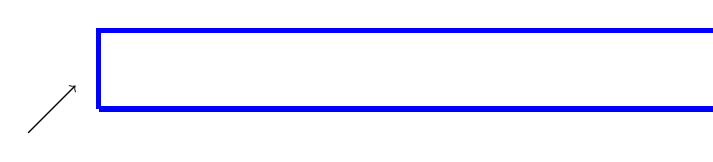
\begin{tikzpicture}
        \creategrid{10}{3}
        \drawobstacle{4}{1}
        \drawobstacle{5}{1}
        \drawobstacle{7}{2}
%        \drawobstacle{7}{4}
%        \drawobstacle{6}{4}
%        \drawobstacle{3}{7}
%        \drawobstacle{2}{2}
%        \drawobstacle{3}{2}
        \draw[->] (0.7,0.7) -- (1.3,1.3);
        \drawgridnode{2}{2}{$N$}
        \drawgridnode{1}{1}{$P$}
%        \drawgridnode{7}{5}{$Z$}
        \drawgridnode{3}{2}{{\color{red} 1}}
        \drawgridnode{2}{1}{{\color{red} 2}}
        \drawgridnode{2}{3}{{\color{red} 3}}
        \drawgridnode{4}{2}{{\color{red} 4}}
        \drawgridnode{3}{1}{{\color{red} 5}}
        \drawgridnode{3}{3}{{\color{red} 6}}
        \drawgridnode{5}{2}{{\color{red} 7}}
        \drawgridnode{4}{1}{{\color{red} 8}}
        \drawgridnode{4}{3}{{\color{red} 9}}
        \draw[blue,line width=2pt] (1,1) -- (9,1) -- (9,2) -- (1,2) -- (1,1);
      \end{tikzpicture}%
    }
  %\end{center}
  \caption{\small 
A current search state (the grid is assumed larger than the part presented).
The red numbers show in which order the traversability of the nodes is tested.
The blue rectangle represents the byte that is returned when we scan the
grid to read the value of location $N = \langle 2, 2\rangle$.
}
  \label{fig::gridforblocks}
\end{figure}

For a motivating example, consider the grid presented in 
Figure~\ref{fig::gridforblocks} 
(this is supposed to be a small chunk of a larger grid).  
The node currently being explored is $N = \langle 2,2\rangle$ 
and its parent is $P = \langle 1,1\rangle$.  
At this stage, the horizontal and vertical axes must be scanned 
for jump points before another diagonal move is taken.  
As it turns out, a jump point will be found at location $\langle 6,2\rangle$.  
When looking for a horizontal jump point on row~$2$, Jump Point Search will 
scan the grid more or less in the order given by the numbers in red, 
depending on the actual implementation.  
Each one of these nodes will be individually tested and each test
involves reading a separate value from the grid.

We will exploit the fact that memory entries are organised into fixed-size 
lines of contiguous bytes. Thus, when we scan the grid to read the value of 
location $N = \langle 2, 2\rangle$ we would like to be returned a byte $B_N$
that contains other bit-values too, such as those for locations up to
$\langle 2, 9\rangle$. In this case we have:
\begin{equation}
B_{N} = [0,0,0,0,0,1,0,0]
\end{equation}
Each zero valued bit in $B_N$ represents a traversable node and each set bit
represents an obstacle.  Note that in practice we read several bytes at one
time and shift the returned value until the bit corresponding to location
$\langle 2, 2\rangle$ is in the lowest position. In a similar fashion and
using only two further memory operations we can read the values for all nodes
immediately above and immediately below those in byte $B$:
\begin{gather}
B_{\uparrow} = [0, 0, 0, 0, 0, 0, 0, 0]\\
B_{\downarrow} = [0, 0, 1, 1, 0, 0, 0, 0]
\end{gather}

\noindent Note that our implementation uses 32-bit words but for this discussion
we will continue to use 8-bit bytes as they are easier to work with.  

%The advantages of such an approach are immediately obvious: instead of
%reading the individual bit-value of every grid location to test for 
%obstacles we can quickly test an entire set of nodes at one time by checking
%whether the corresponding byte evaluates to zero.
When searching recursively along a given row or column
there are three possible reasons that cause JPS to stop: 
a forced neighbour is found in an adjacent row, a dead-end is 
detected in the current row or the target node is detected in the
current now.
We can easily test for each of these conditions via simple
operations on the bytes $B_{N}, B_{\uparrow}$ and $B_{\downarrow}$.
\\ \noindent
\textbf{Detecting dead-ends:}
A dead-end exists in position $B[i]$ of byte $B$ if $B[i] = 0$ and 
$B[i+1] = 1$. We can test for this in a variety of ways;
CPU architectures such as the Intel x86 family for example have the native 
instruction \texttt{ffs} (find first set). The same instruction is available as
a built-in function of the \textsc{GCC} compiler. When we apply
this function to $B_{N}$ we find a dead-end at position 5.
\\ \noindent
\textbf{Detecting forced neighbours:}
A potential forced neighbour exists in position $i$ of byte $B$, or simply 
$B[i]$, if there is an obstacle at position $B[i-1]$ 
and no obstacle at position $B[i]$. We test for this condition with the
following bitwise operation (assuming left-to-right travel):
\begin{equation}
\texttt{forced(B) = (B\ \& !(B<<1))}
\end{equation}
When we apply this procedure to $B_{\downarrow}$ we find a potential jump 
point at bit position~$3$; $\texttt{forced}(B_{\uparrow})$ yields no potential jump points.

In order to minimise the number of branching instructions (important
to prevent CPU stalling) we do not test the individual results of 
operations: rather we combine their results by way
of bitwise disjunction into a single byte $B_{S}$ (S for stop).
For the example in Figure~\ref{fig::gridforblocks} we have 
\begin{flalign}
B_S &= \mathrm{forced}(B_{\uparrow})\quad|\quad \mathrm{forced}(B_{\downarrow})\quad | \quad B_N & \\
B_S &= [0,0,0,1,0,1,0,0] & 
\end{flalign}

Because $B_S \neq 0$, we know that the search has to stop.  Using the
\texttt{ffs} command we extract the position of the first set bit in $B_S$
(call this bit $b_S$) and compare it with the position of the first set bit
in $B_N$ (call this bit $b_N$).  If $b_S \leq b_N$ we have discovered a jump point at
location $B_N[b_S-1]$; otherwise we have hit a dead-end.  Alternatively, if
$B_S$ evaluates to zero there is no reason to stop: we jump ahead 7 positions
(not 8) and repeat the procedure until termination.
\\ \noindent
\textbf{Detecting the target node:}
To avoid jumping over the target node we compare its position to the position
of the node where the block-based symmetry-breaking procedure terminated --
either due to finding a successor or a reaching dead-end. If the target lies
between these two locations we generate it as any other jump point successor.

\subsection*{Additional Considerations}
The procedure we have described in our running example is applicable in the case
where JPS scans the grid left-to-right. The modification for right-to-left
scanning is simple: we shift the current node into the most significant position
of $B_N$ and replace \texttt{ffs} with the analogous instruction \texttt{msb}.  In the case
of up-down travel we have found helpful to store a redundant copy of the
map that is rotated by 90 degrees. Other possibilities also exist that do not
incur an overhead: for example the map may be stored as blocks of size $m
\times n$ that each contain bits from several rows and columns. Such an
approach would also benefit diagonal travel (which in our implementation
remains step-by-step) but may reduce the step size during horizontal scanning.
%
%whether an 
%
%The status of the eight nodes in the blue rectangle 
%starting from $\langle x,y\rangle = \langle 2,2\rangle$ in the figure 
%could for instance be represented by a single byte 
%$B = [0,0,0,0,0,1,0,0]$ 
%whereby the $i$th bit $B[i]$ of the byte is set to $1$ 
%iff the node $\langle x+i,y\rangle$ of the grid contains an obstacle.  
%(Practically, the implementation uses 32-bit words, 
%but this discussion will stick to 8-bit bytes for simplicity.)
%In particular, it would be easy to see that the block 
%between $\langle 2,3\rangle$ and $\langle 9,3\rangle$ 
%is obstacle-free because the corresponding byte evaluates to $0$.  
%
%More generally, we can build a byte $B_S$ 
%which will represent the list of positions 
%at which the agent must stop.  
%If this byte evaluates to $0$, 
%we can jump $7$ steps (here, to $\langle 9,2\rangle$) 
%and keep searching for the next $8$ cells.  
%
%

%EOF 
